\subsection{DCGAN}
\label{sec:exp-dcgan}

We implement our baseline model in this section. The DCGAN is evaluated on cifar10. We present the evolution of the inception score in Figure \ref{fig:exp-dcgan-is} and both losses in Figure \ref{fig:exp-dcgan-losses}
   
\begin{figure}[t!]
    \centering
    \begin{subfigure}[t]{0.49\textwidth}
        \centering
		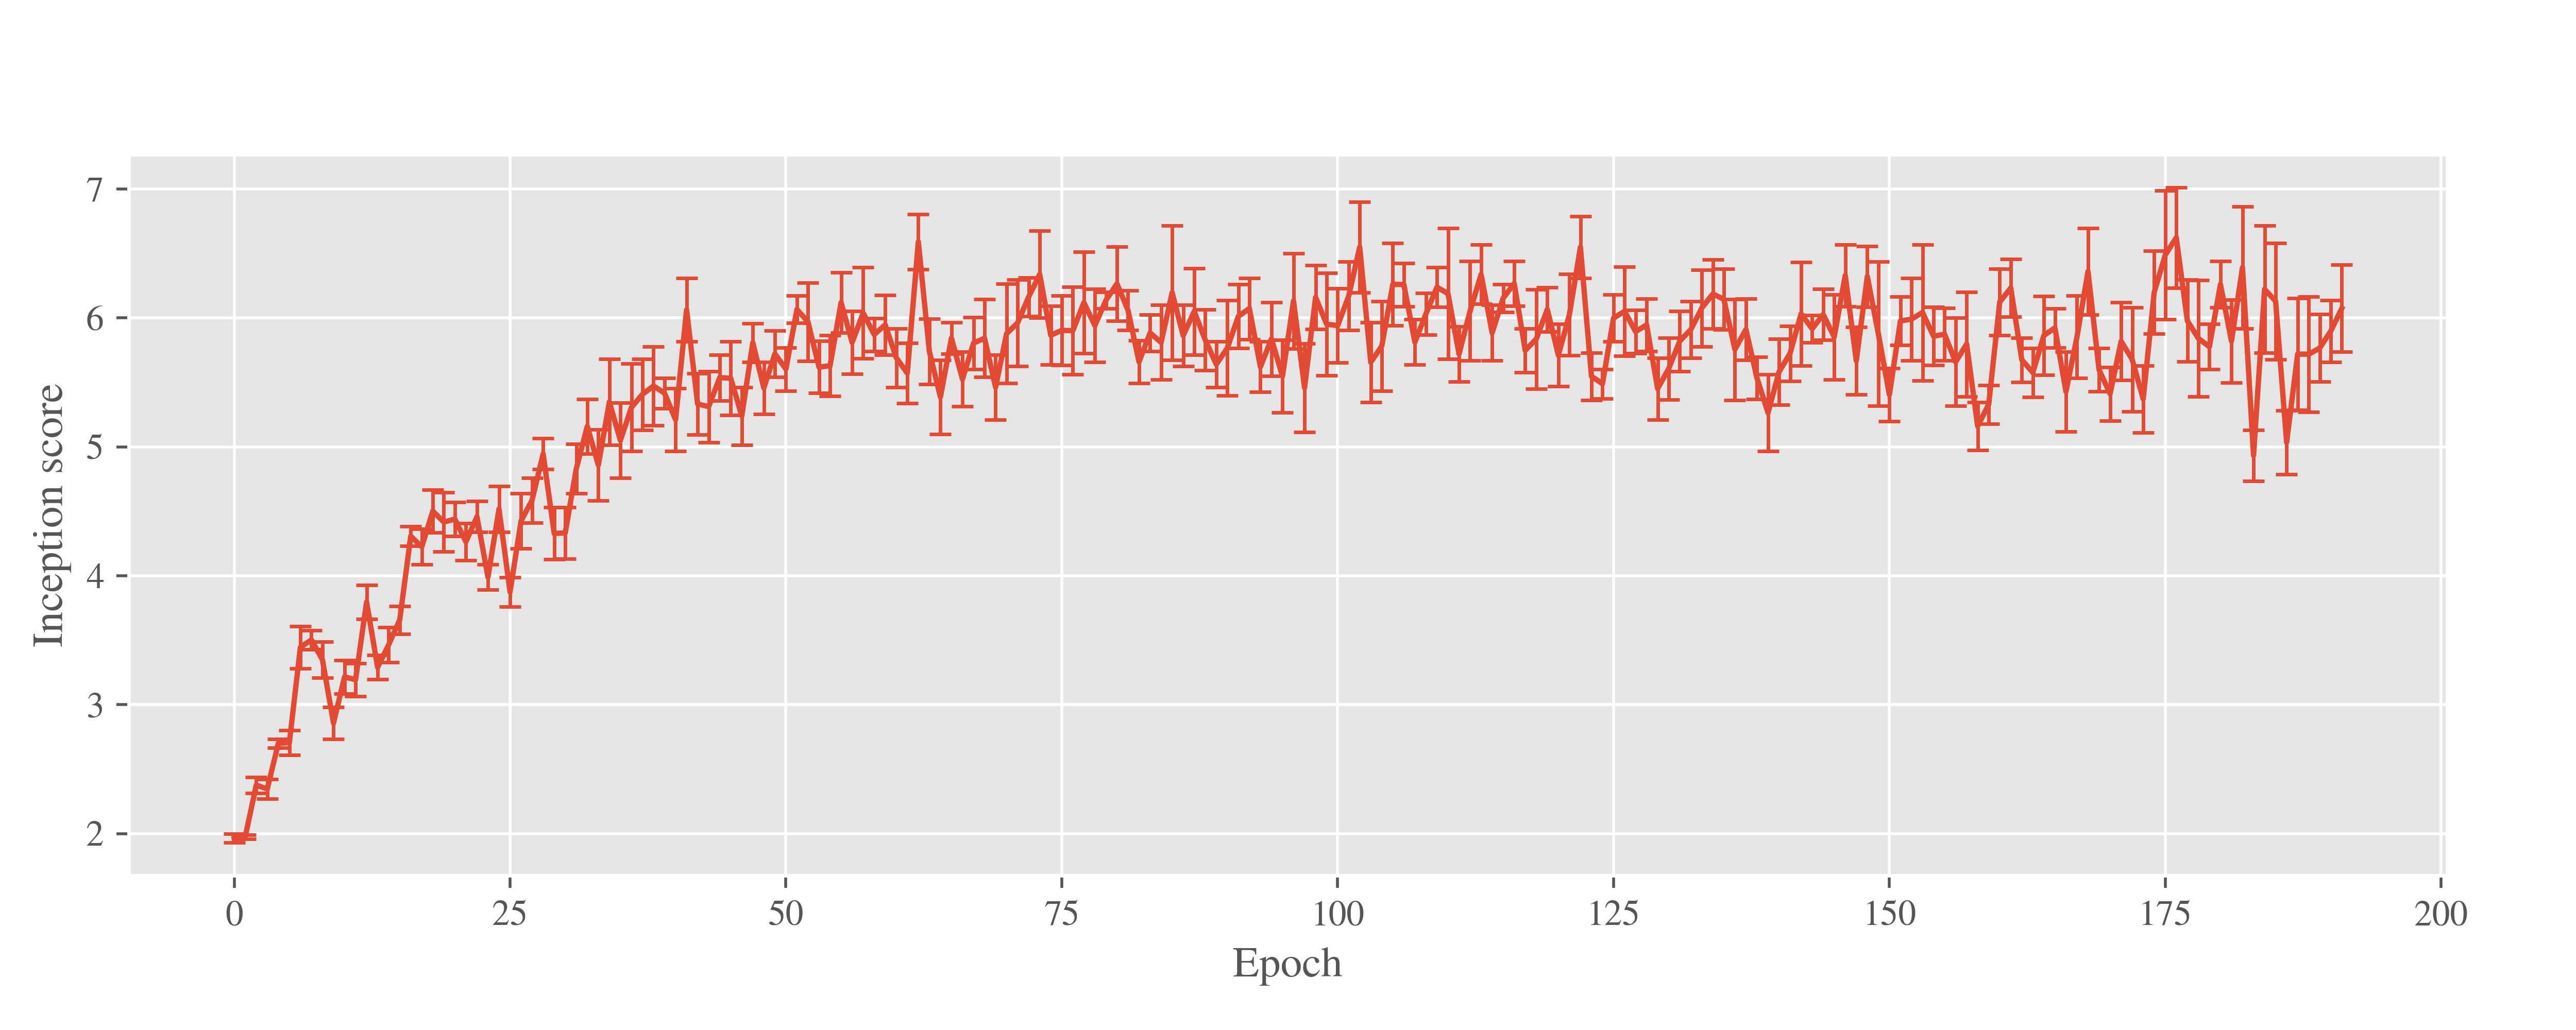
\includegraphics[width=\textwidth]{../code/results/figures/dcgan_cifar10_is.png}
		\caption{Inception score}
		\label{fig:exp-dcgan-is}
    \end{subfigure}
    \begin{subfigure}[t]{0.49\textwidth}
        \centering
        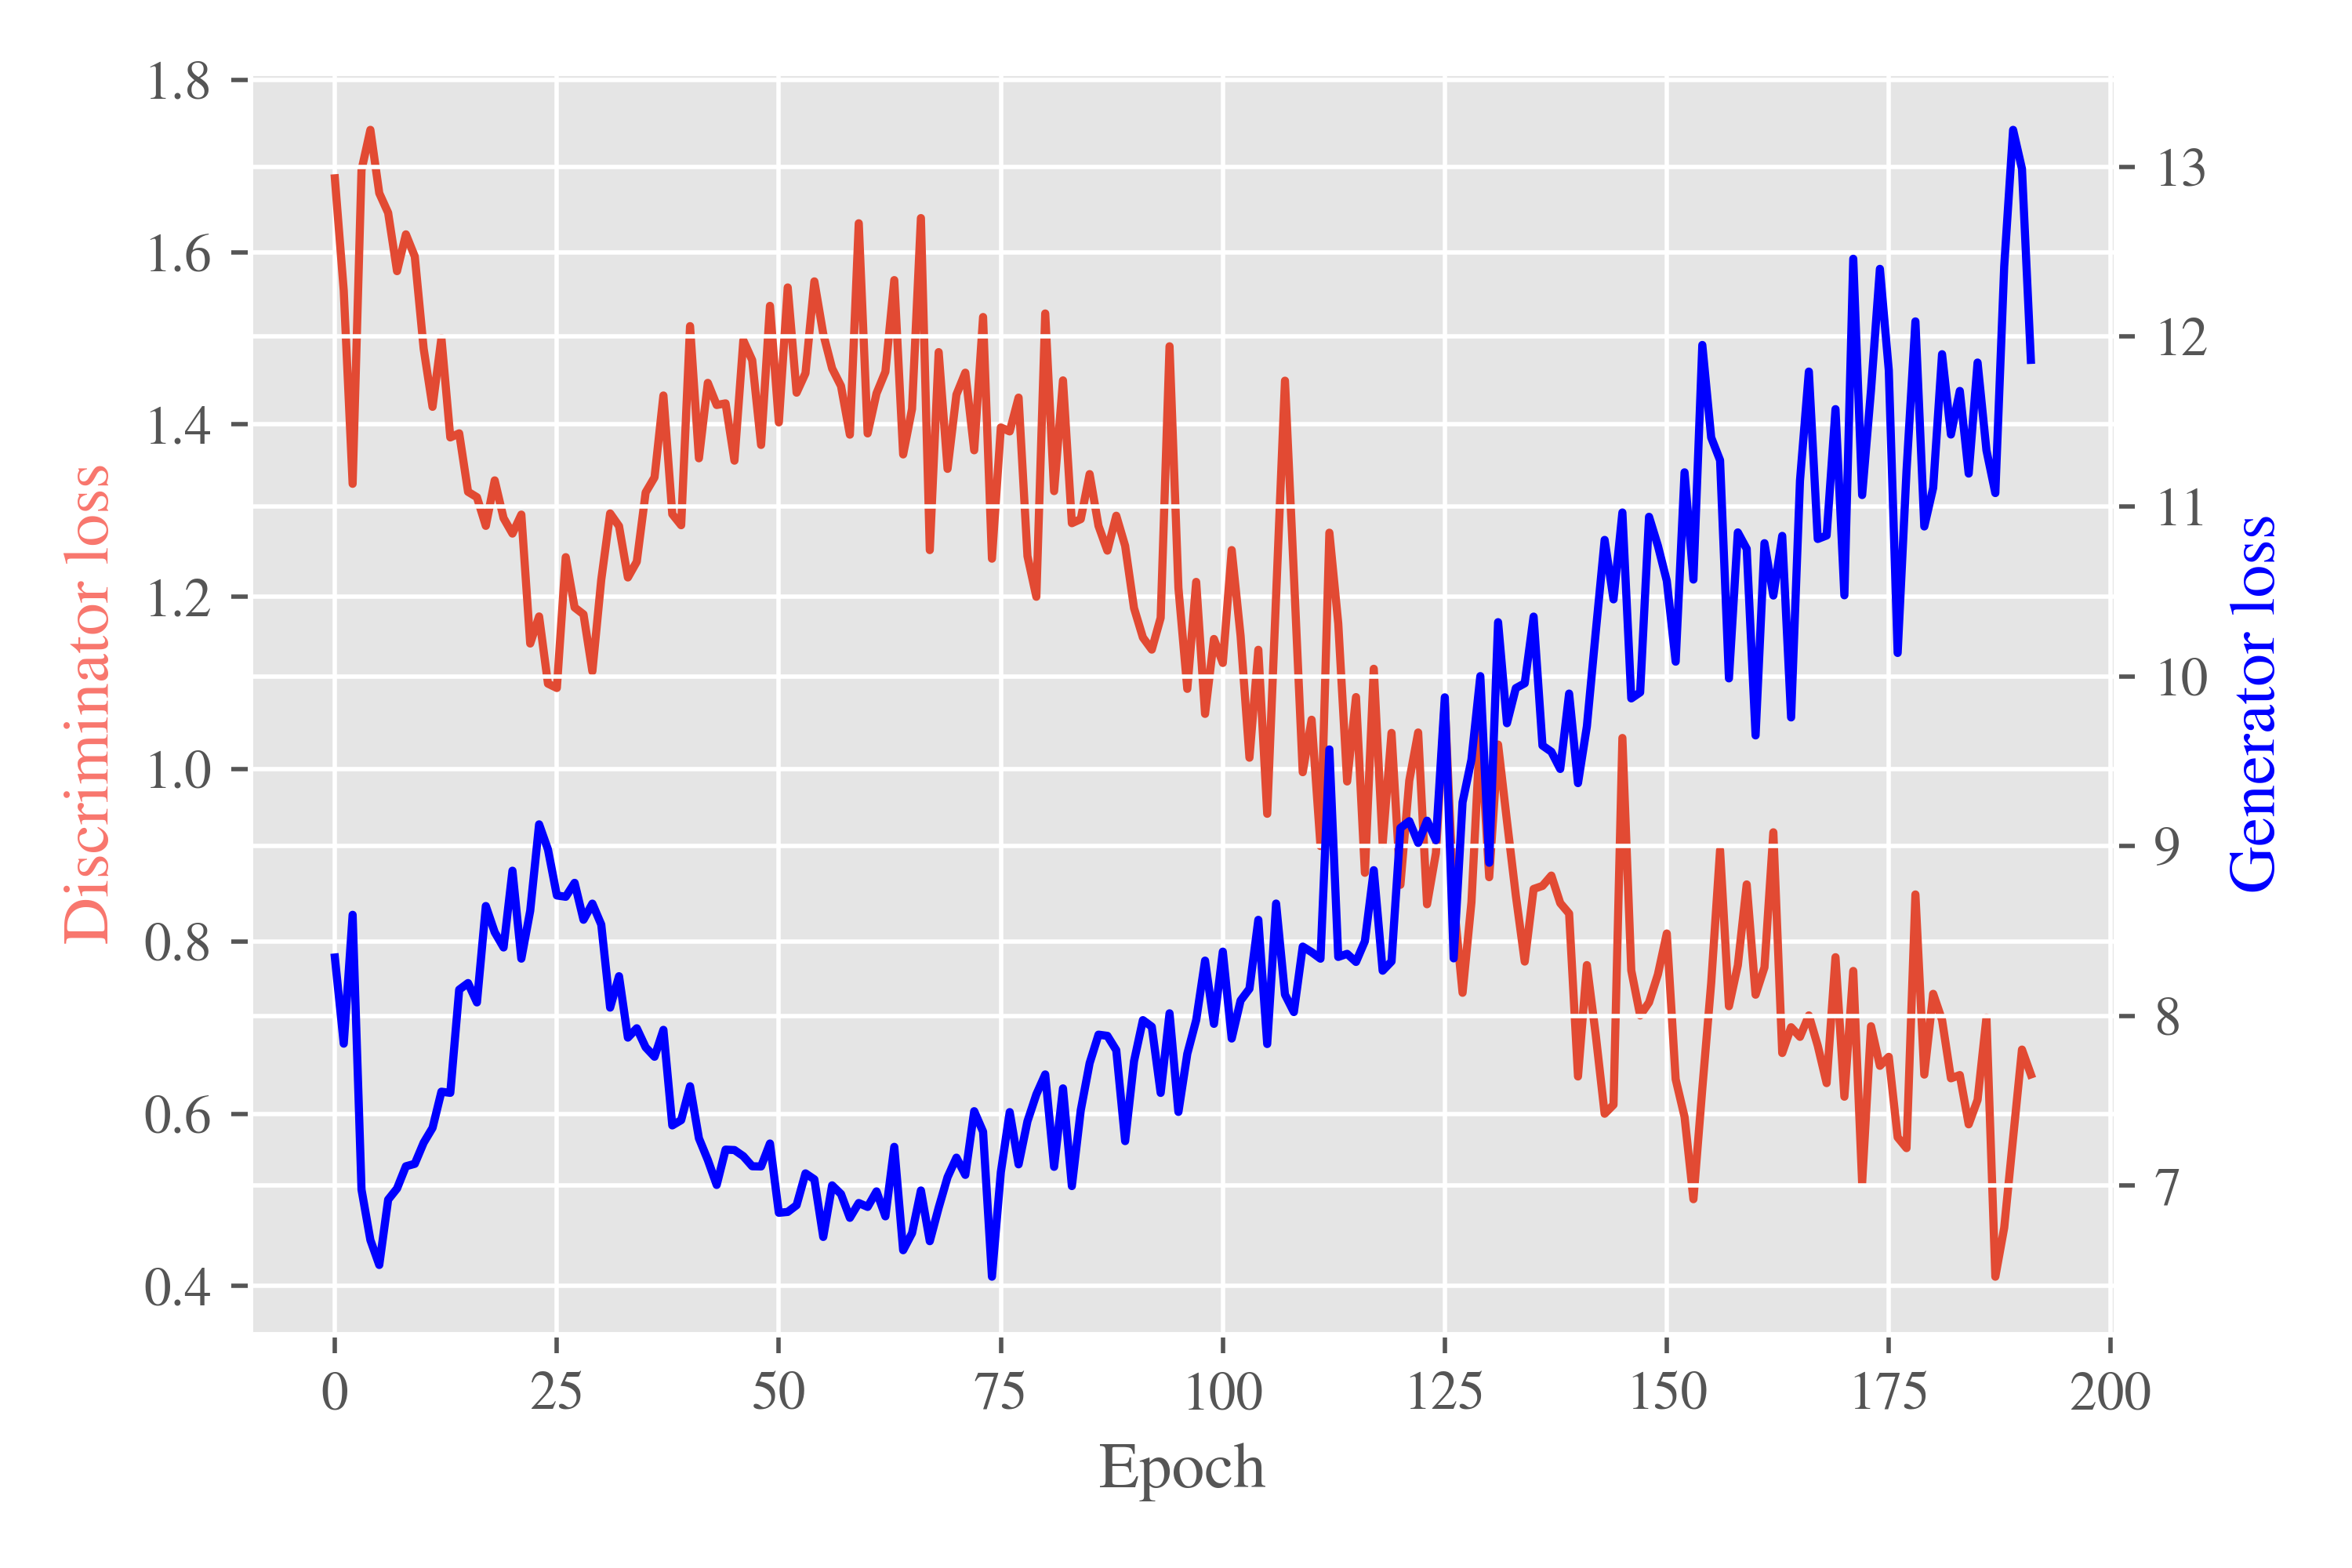
\includegraphics[width=\textwidth]{../code/results/figures/dcgan_cifar10_losses.png}
		\caption{Losses}
		\label{fig:exp-dcgan-losses}
    \end{subfigure}
    \caption{DCGAN - training on CIFAR10 over 190 epochs.}
\end{figure}

Losses can hardly be interpreted when treating with GANs, since the generator and discriminator are in a situation of competition where an improvement on the one leads to a deterioration on the other.

